% \include{preamble}
\documentclass[12pt]{article}
\usepackage{siunitx}
\usepackage{calc}
\usepackage{xfp}
\usepackage{enumitem}
\usepackage[a4paper]{geometry}
\usepackage{ragged2e}
\usepackage{xcolor}
\usepackage{sectsty}
\usepackage{fontspec}
\usepackage{mathspec}
\usepackage{ebgaramond}
\usepackage{lipsum}
\usepackage{eso-pic}
\usepackage{graphicx}
\usepackage{svg}
\usepackage{xfp}
\usepackage{marginnote}
\usepackage[backend=bibtex]{biblatex}
\addbibresource{resources.bib}
\usepackage{floatrow}
\usepackage[
  colorlinks=true,
  linkcolor=black!70,
  citecolor=goldenrod,
  urlcolor=black!70
]{hyperref}
\usepackage{cleveref}

\crefformat{figure}{\textcolor{goldenrod}{\textsc{f#1}}}
\Crefname{figure}{\textcolor{goldenrod}{\textsc{f}}}{\textcolor{goldenrod}{\textsc{f}}}

% colored citations
\DeclareCiteCommand{\cite}
  {\usebibmacro{prenote}}
  {\href{#1}{\textcolor{goldenrod}{[\usebibmacro{citeindex}\usebibmacro{cite}]}}}
  {\multicitedelim}
  {\usebibmacro{postnote}}
  
\usepackage{xcolor}
\definecolor{goldenrod}{HTML}{B8860B}
\usepackage{caption}
\DeclareCaptionLabelFormat{custom}{\textcolor{goldenrod}{\textsc{f#2 |}}}
\captionsetup[figure]{
  labelformat=custom,
  labelsep=space,
  font=footnotesize,
  textfont={color=black!60}
}
\usepackage{fancyhdr}
\pagestyle{fancy}
\fancyhf{}


\fancyfoot[RO,LE]{\thepage}
\renewcommand{\headrulewidth}{0pt}
\renewcommand{\footrulewidth}{0pt}

\newcommand{\PHI}{\fpeval{(1 + sqrt(5)) / 2}}
\newcommand{\INVPHI}{\fpeval{2/(1 + sqrt(5))}}

\setlist[enumerate]{%
  topsep = {\INVPHI}em,
  leftmargin = {\PHI}em,
  rightmargin = {\PHI}em,
  itemsep = 0em
}


\geometry{
  top=36mm,
  bottom=36mm,
  left=37mm,
  right=59mm,
  headheight=15pt,
  headsep=12pt,
  footskip=20pt
}

\setlength{\marginparwidth}{3cm} 
\setlength{\marginparsep}{3em} 


\allsectionsfont{\normalfont\itshape}






%%%%%%%%%%%%%%%%%%%%%%%%%%%%%%%%%%%%%%%%%%%%%%%%%%%%%%%%%%%%%%%%%%%%%%%%%%%%%%%%%%%%%%%%%%%%%%%%%%%%
\begin{document}

    \setmathfont{Garamond-Math.otf}
    \RaggedRight
    \setlength{\parindent}{1em}

\clearpage
\AddToShipoutPictureBG*{%
  \put(220,-620){\scalebox{-1}[1]{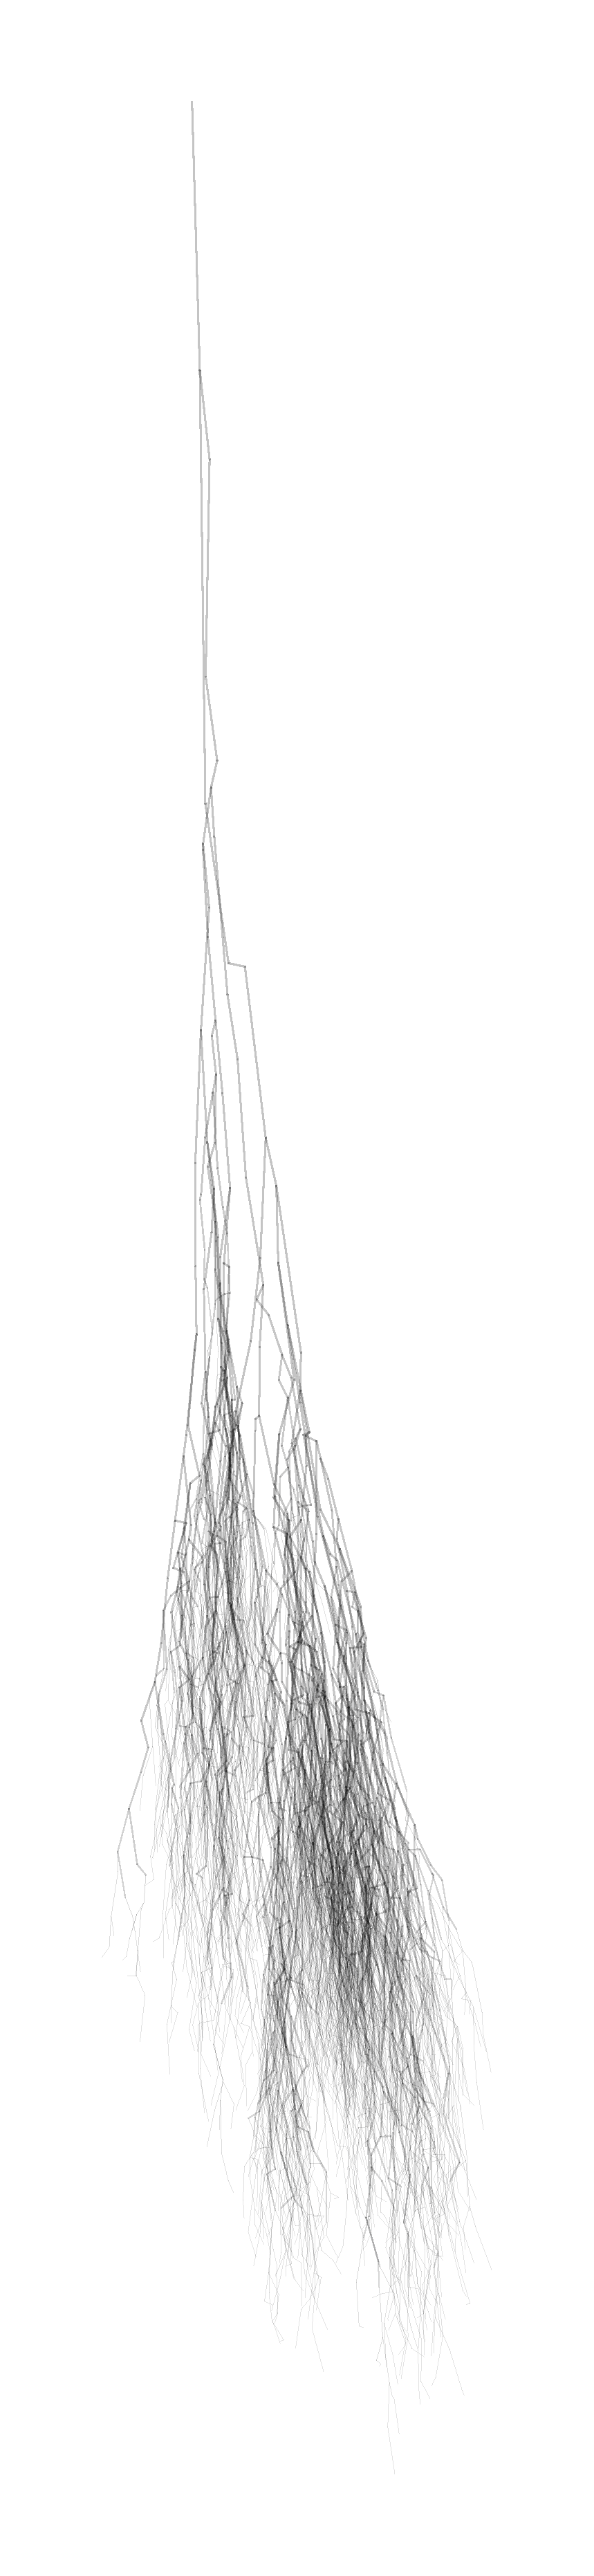
\includegraphics[height=250em]{images/shower.pdf}}}%
}
\thispagestyle{empty}
    \color{black!80}
    \begin{flushleft}
        \raggedright
        \vspace*{14em}
        \huge \textit{Conceptual design report} \\[0.3em]
        \normalsize \textsc{phys 494 / iarc 425 — design \& cosmic rays} \\[3em]
        \normalsize{
            Micah Hillman \hspace{0.8em} Hunter Whitley \hspace{0.8em} Eliza Berrong \hspace{0.8em} Jaedyn Florence\\[0.3em]
        }
        \vspace{12em}
        \normalsize\color{black!70} \today
    \end{flushleft}
\clearpage
\AddToShipoutPictureBG*{}  % Clear background for next pages

    \pagebreak
    \section{Introduction}\label{sec:intro}
    \textsc{throughout the semester} (Spring 2025), we have focused our efforts on fostering a deep interdisciplinary collaboration between physics and design students, exploring the phenomenology of \textit{cosmic rays}—a blend of exotic and ordinary particles formed by high-energy cosmic events. The life of a cosmic ray generally unfolds in two stages:
    \begin{enumerate}
        \item   a \textit{progenitor}—most commonly a proton—is produced in a high-energy astrophysical process (\textit{e.g.}, a supernova, an active galactic nucleus | \textsc{agn}, colliding galaxies, and so on);
        \item through random collisions with atmospheric matter, the progenitor's energy splinters into a shower of \textit{new particles} (including pions, muons [from the decay of pions], electrons/positrons, neutrinos, and many others).
    \end{enumerate}
    This process results in the prolific synthesis of numerous fundamental particles—most of which are practically invisible—which, in humanity's long history, we have only recently been able to detect. (There are very few means by which a person could directly sense a cosmic ray, but it is known that the interaction of high-energy neutrinos with water produces a transient ``click'' in the range of 10 kHz—well within the range of human hearing; however, you'd have to be very lucky to be in the right place and time to sense it. Even then, the sound is very similar to the snapping of pistol shrimp!) Cosmic rays are corpuscles of deep universal truth; studying them in detail allows us to gain insights into the nature of universal laws. 
    
    Many of the facets of nature on display in cosmic showers are the same ones that are wielded by scientists and engineers working on what have been referred to as ``the world's machines''—particle colliders like the Large Hadron Collider | \textsc{lhc} at \textsc{cern} along the Franco–Swiss border, which intentionally create high-energy particle collisions in order to synthesize and study new particle interactions. Still, the energies produced at these humble human machines are puny compared to many cosmic rays.

    This collaboration's primary goal was to bring greater understanding and awe of these cosmic phenomena to the general public by designing a modular prototype for making these phenomena \textit{experiential}—that is, bringing them into the realm of human perception by creative means. Our design took the form of a stochastically-driven audiovisual experience meant to symbolize (moreso than manifest) direct experience of cosmic phenomena. 

    \pagebreak
    \section{Investigative process}

    \textsc{to find footing} at the science–design interface, we explored a number of different precedent works. Notably, \textit{A Touch of Code}~\cite{Klanten2011ATO} introduced us to the world of code-oriented design; the projects in this book directly influenced our thinking and ultimate design process while creating electronic components and code interfaces for our design. For the designers in our group, an exploration of the work of Robert Irwin (1928–2023)~\cite{weschler1982seeing}—a pivotal figure in the \textit{Light and Space} movement—provided a philosophical basis for much of our work; his emphasis on light manipulation was reflected in our final design (see~\cref{fig:irwin}). 
    \begin{figure}[h]
        \floatbox[{\capbeside\thisfloatsetup{capbesideposition={right,center},capbesidewidth=3.5cm}}]{figure}[\FBwidth]
        {\caption{Robert Irwin, \textit{Multiple Configurations \#1}, 2018, acrylic~\cite{irwin2018multiple}.}\label{fig:irwin}}
        {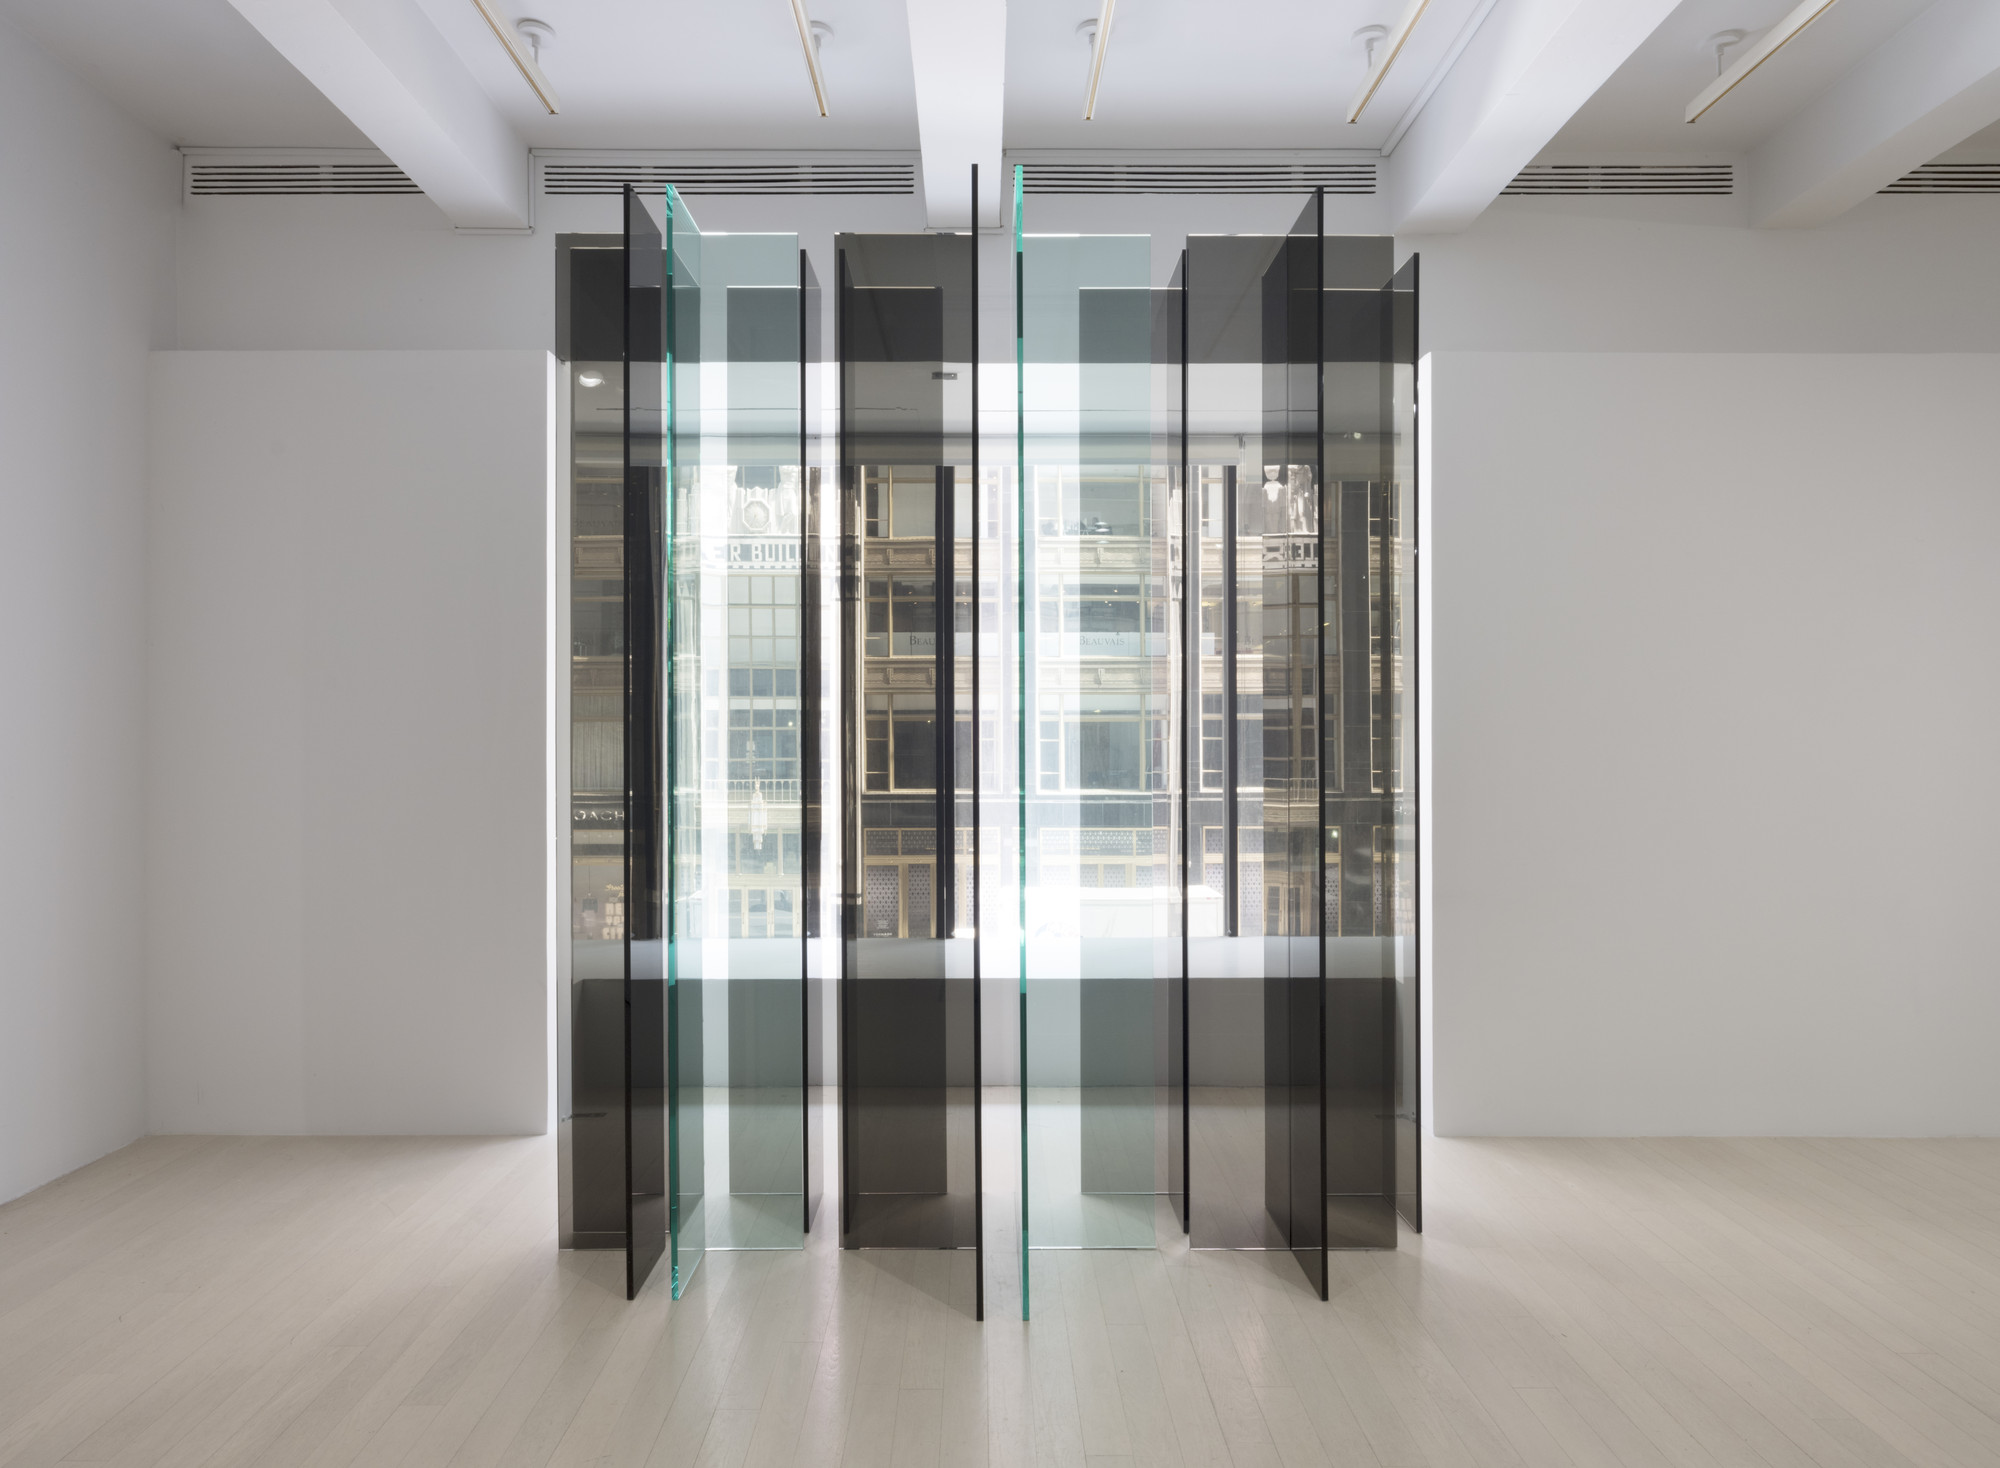
\includegraphics[width=\linewidth]{images/irwin.png}}
    \end{figure}
    Much of the precedent study in preliminary stages of the design process also involved the creation of shared vision-boards and the collection of various inspirational media. We were captivated early on by the idea of exploring cosmic rays in infinitely-mirrored spaces (see~\cref{fig:infinity mirror}), inspired by a cloud chamber viewing on the first day of class.
    
    \begin{figure}[h]
        \floatbox[{\capbeside\thisfloatsetup{capbesideposition={left,center},capbesidewidth=3.5cm}}]{figure}[\FBwidth]
        {\caption{An infinity mirror box. The optical effect shown is created by mutually facing semitransparent mirrored surfaces at one another, resulting in a vicious cycle of internal light reflection. Some amount of light escapes the loop at each reflection, and that is what we see.}\label{fig:infinity mirror}}
        {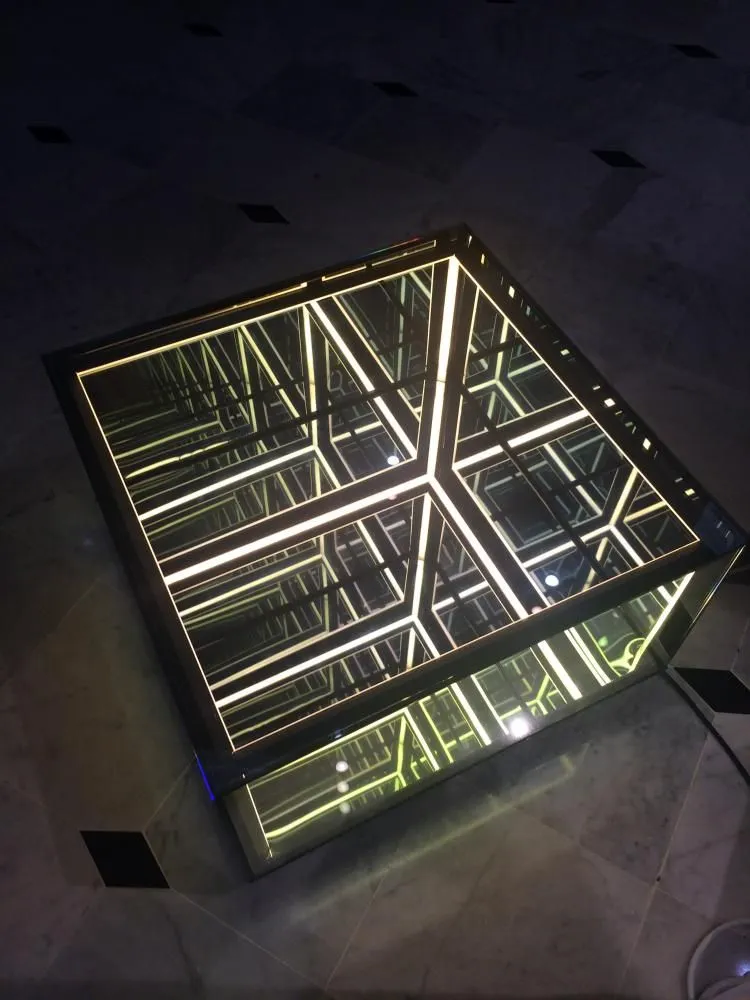
\includegraphics[width=\linewidth]{images/mirrorbox.png}}
    \end{figure}

    With these newfound bearings and a catalyzing idea to carry us forward, we set out developing our project.
    
    \pagebreak
    \subsection{Concept development}

    Prototyping was constrained to fit within a one-cubic-foot box. Initially, we were unsure what kind of project to pursue (other than, of course, an infinitely-mirrored box), so we began with a simple goal: create something modular, allowing ourselves flexibility to explore different configurations within the constraints. The process evolved organically and incrementally, beginning with the development of a basic modular series of connectors (\cref{fig:connectors}), which we iteratively refined as new ideas emerged and the direction of the project became clearer.

    \begin{figure}[h]
        \floatbox[{\capbeside\thisfloatsetup{capbesideposition={left,center},capbesidewidth=3.5cm}}]{figure}[\FBwidth]
        {\caption{A set of 3D-modeled connector pieces was developed to give ourselves Lego-like building blocks to work with while designing. They gave us a workspace for material–light exploration.}\label{fig:connectors}}
        {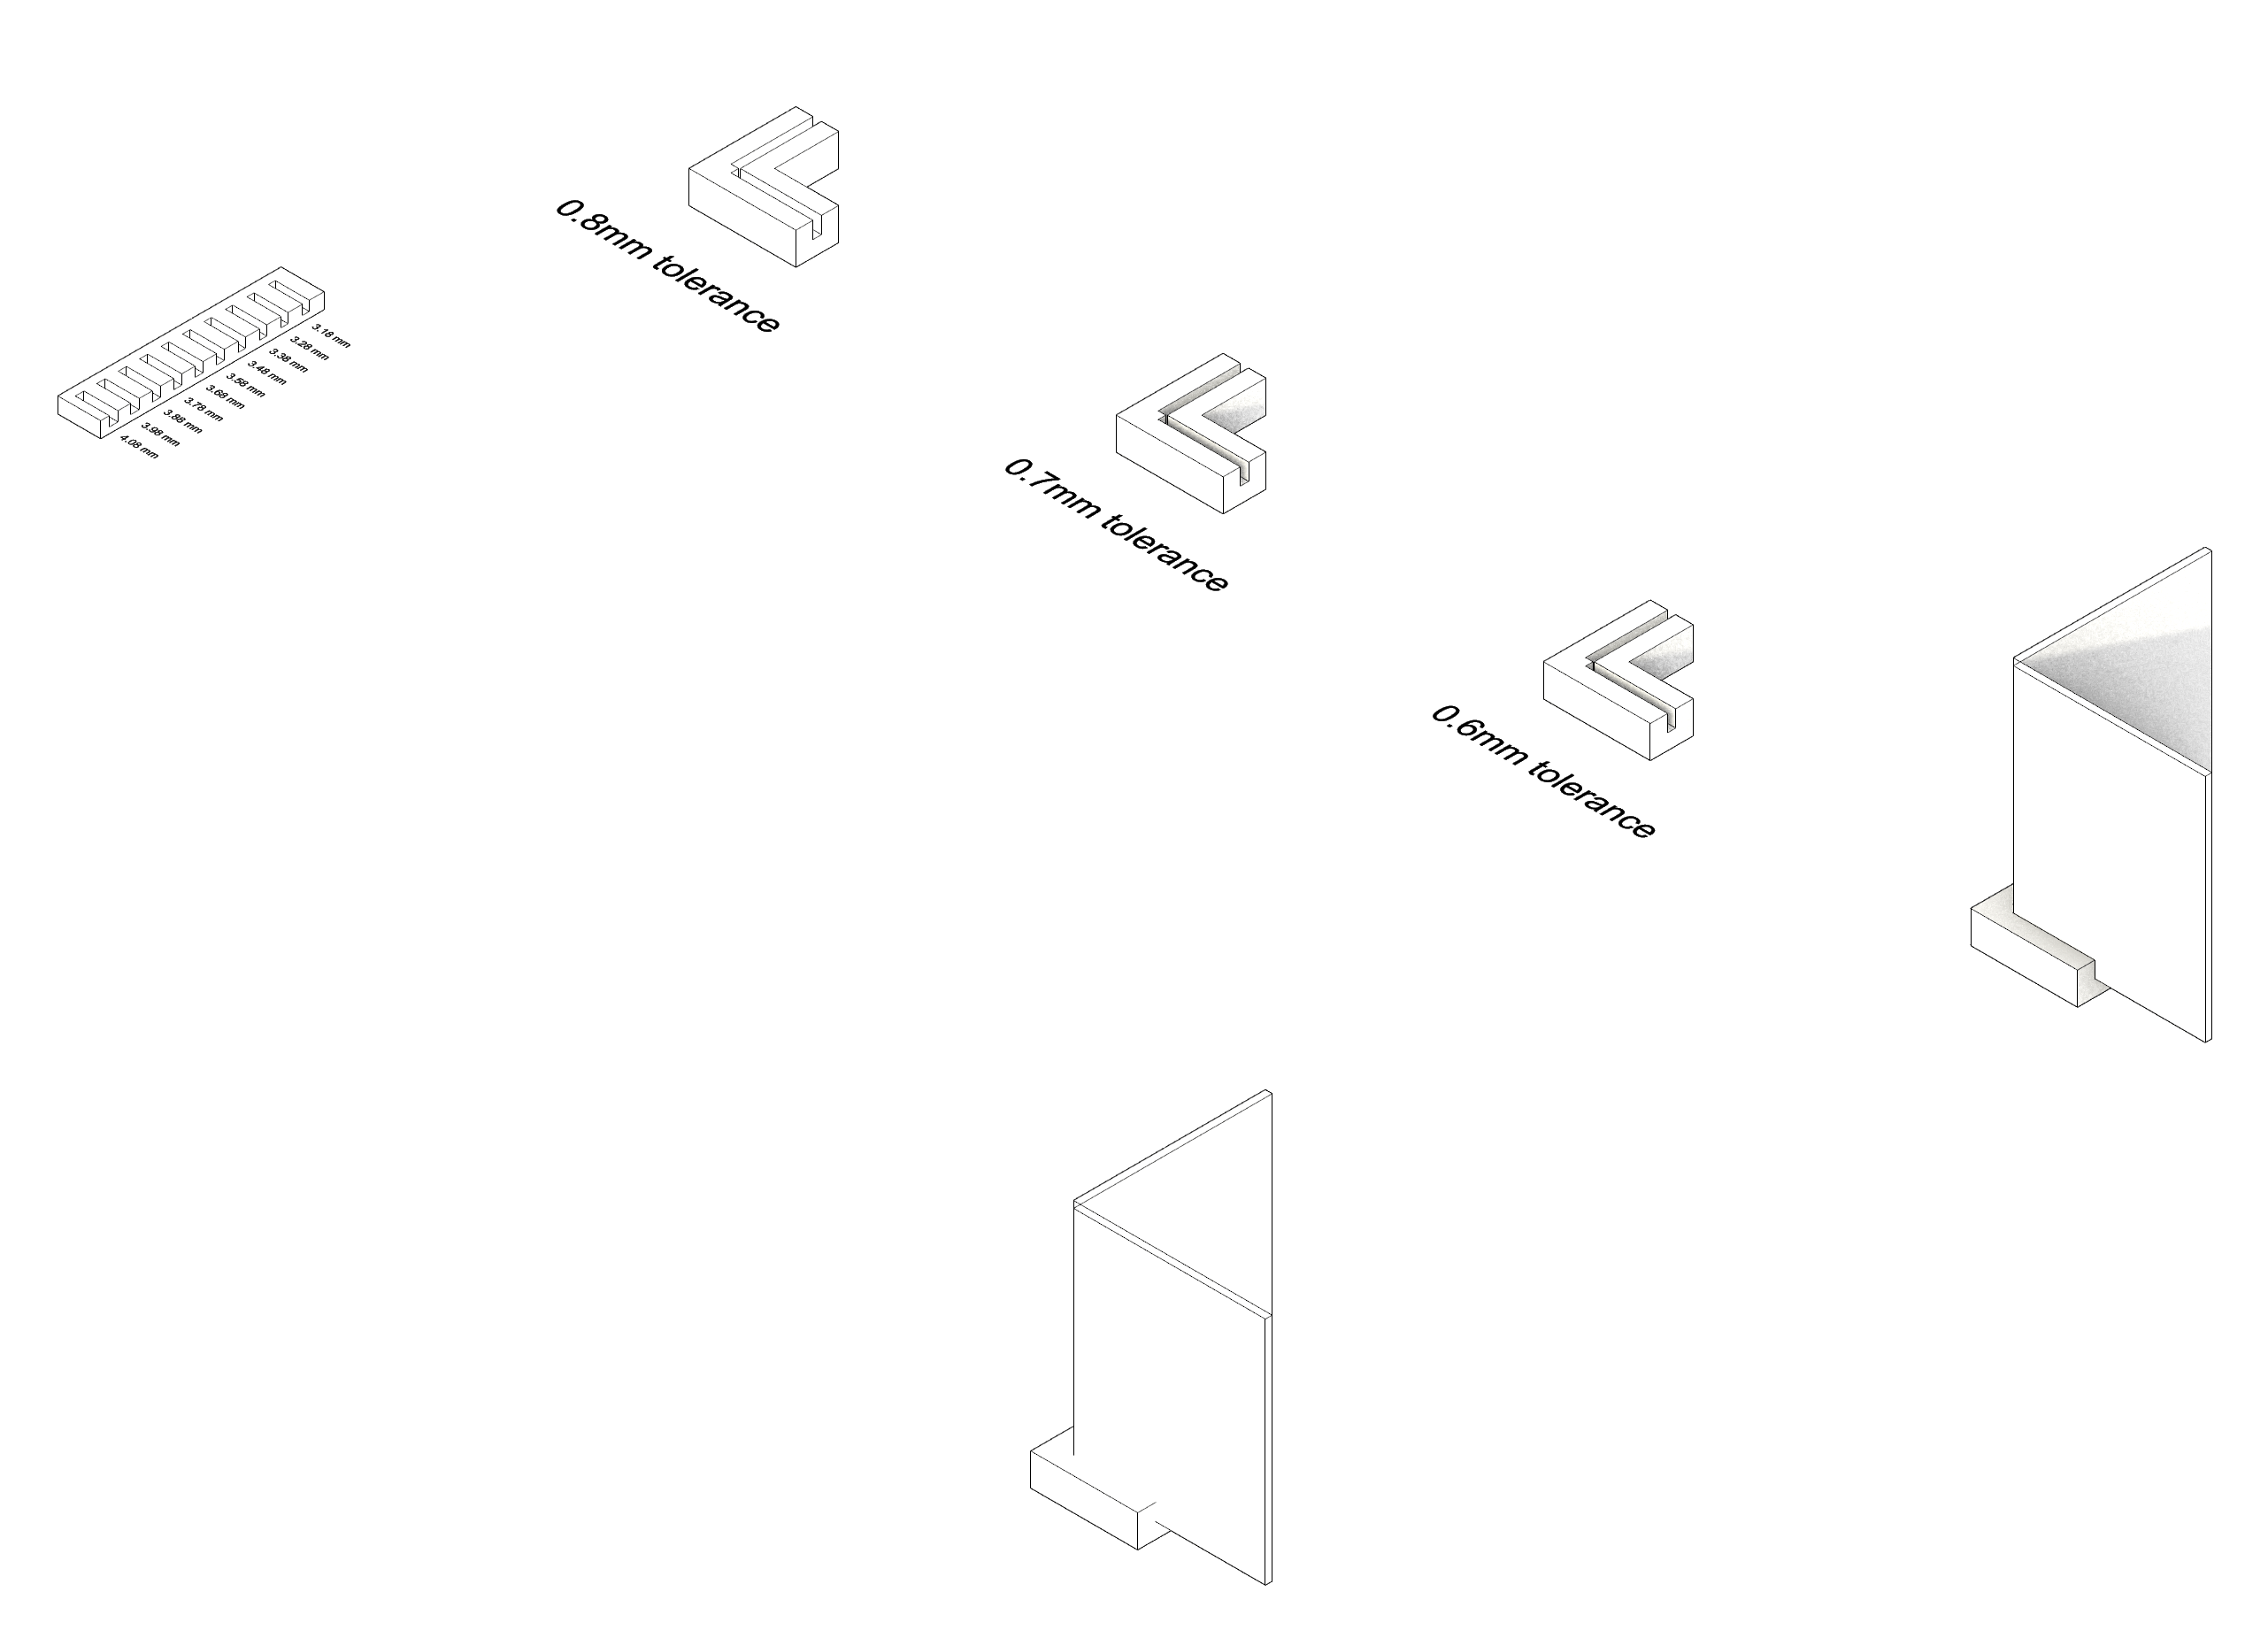
\includegraphics[width=12cm]{images/connectors.png}}
    \end{figure}

    \begin{figure}[h]
        \floatbox[{\capbeside\thisfloatsetup{capbesideposition={right,center},capbesidewidth=7cm}}]{figure}[\FBwidth]
        {\caption{Imagined assembly of connector pieces with sheets of plexiglass. This iteration relied on horizontal orientation for stability; later iterations were symmetric about the vertices (cubical, rather than planar as shown here).}\label{fig:assembled}}
        {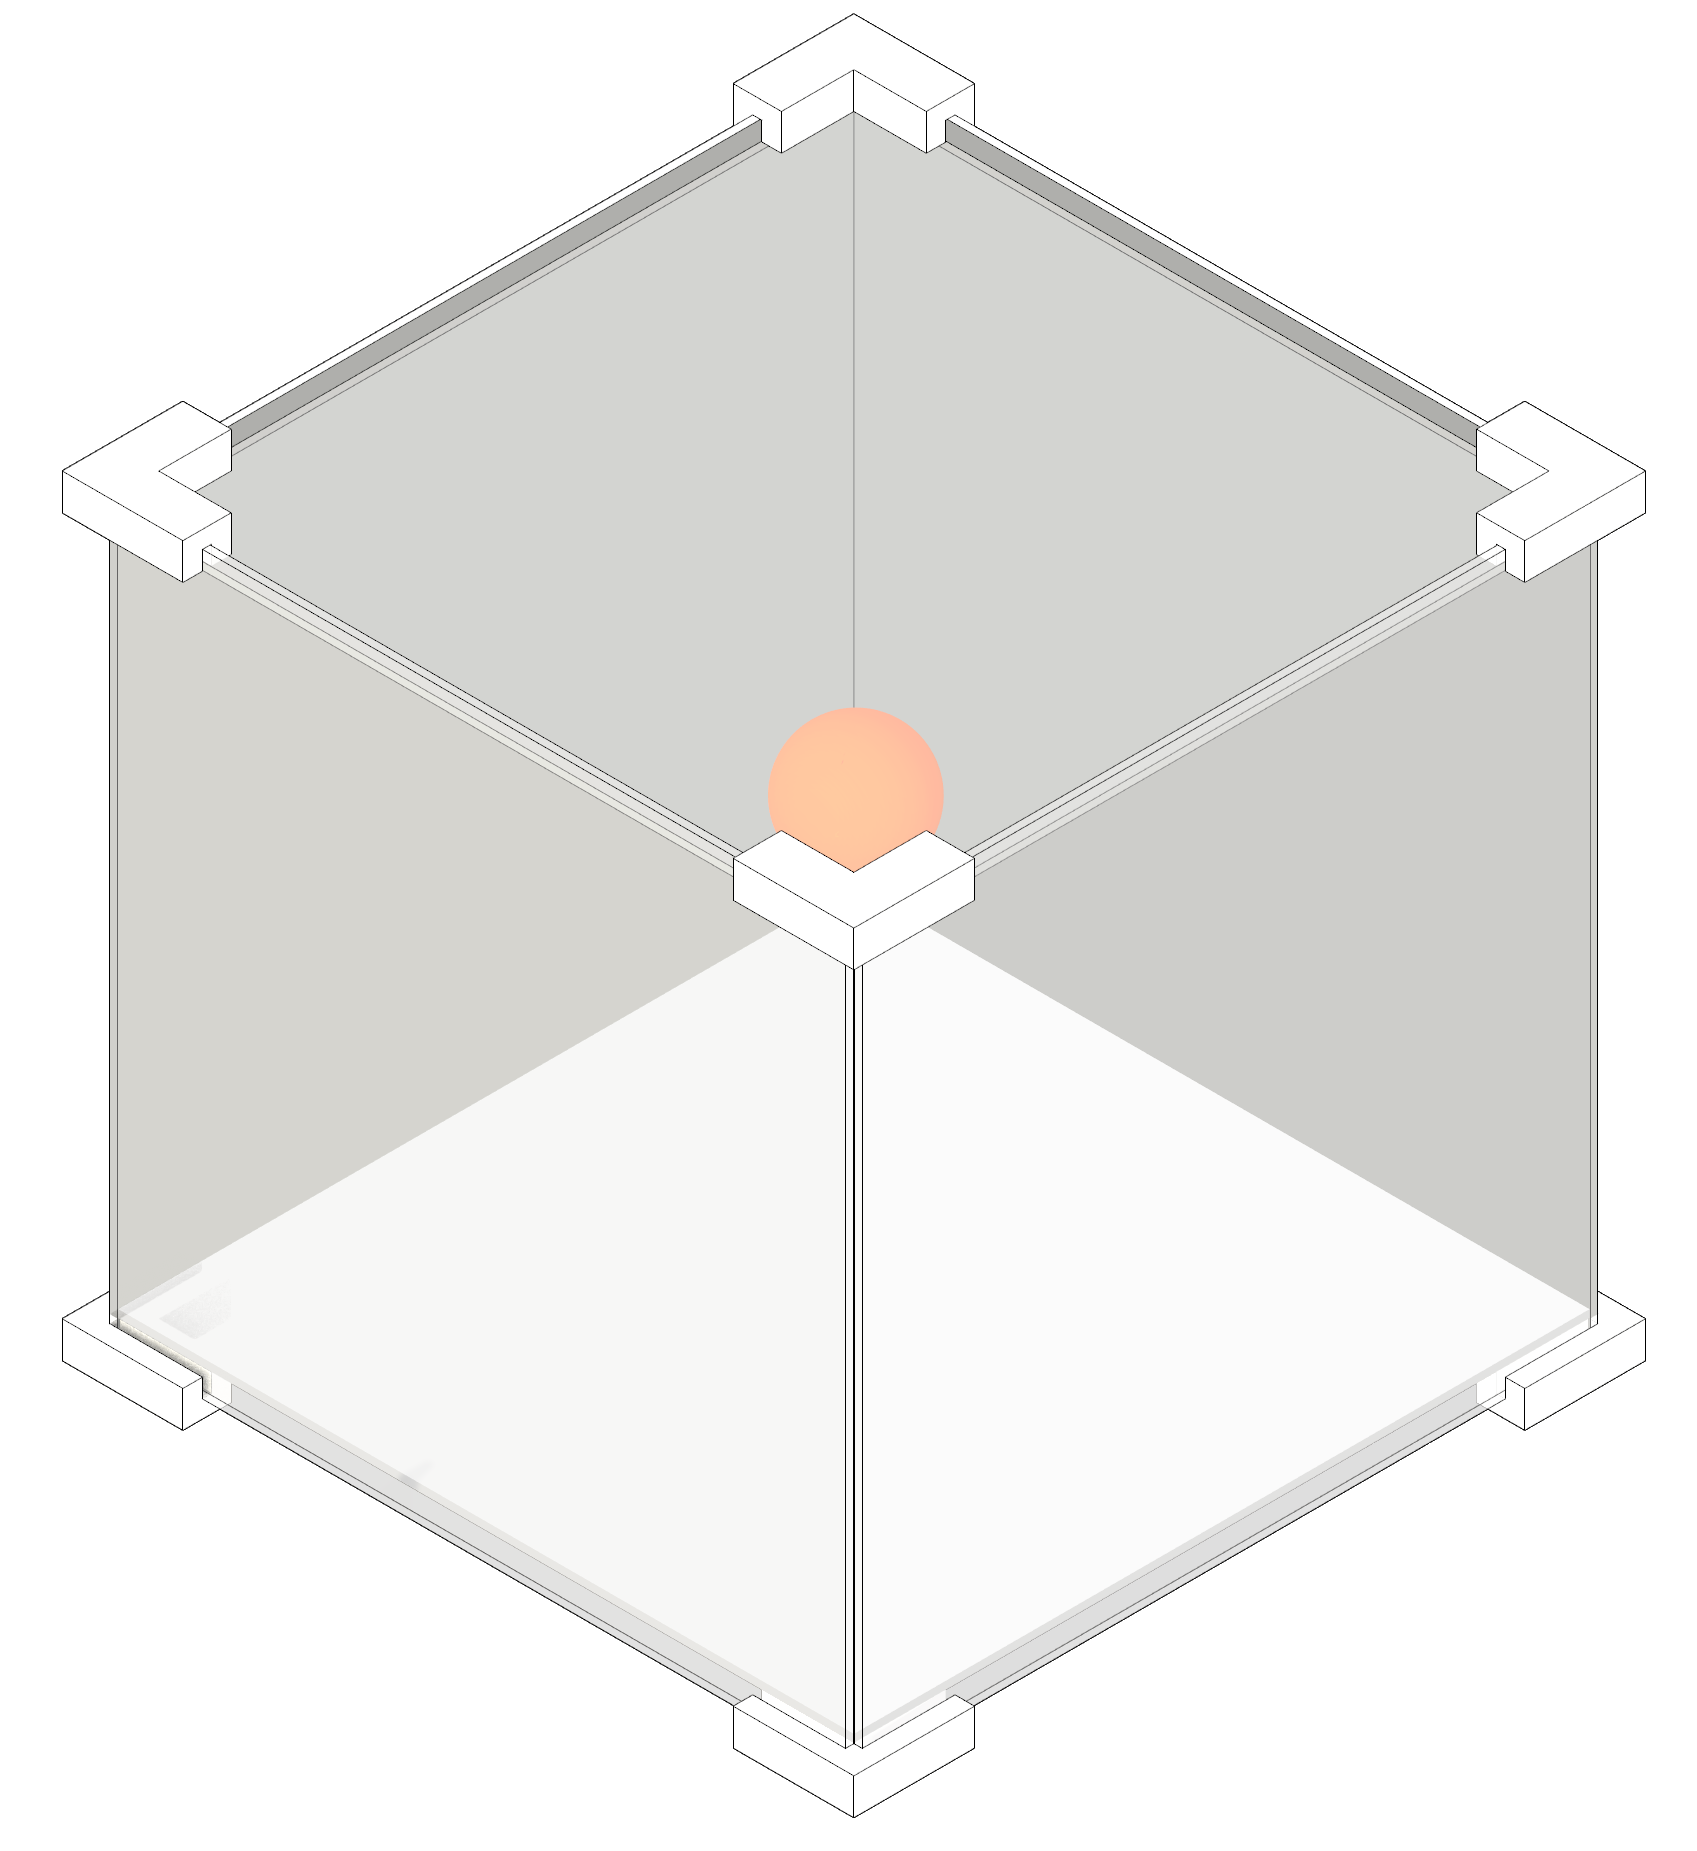
\includegraphics[width=6.8cm]{images/assembled.png}}
    \end{figure}

    Over time, we recognized the need for more immersive elements. Knowing that lighting was essential to a more immersive and awe-inspiring experience, we opted for a simple Arduino–\textsc{led} setup running with a simple test script to provide a light source. This setup was sufficiently modular to allow for hot-swapping of addressable \textsc{led} strips; we experimented with both linear and planar configurations. Eventually, we developed our own program—one which stochastically generated points of light, accelerating them down our \textsc{led} strip of choice. The acceleration effect was more pronounced with longer strips, but we ultimately selected a series of shorter strips to pair with another further iteration... Sound!

    We decided to make our project more immersive using a process akin to \textit{sonification} (complementing numerical or visual data with a non-speech sound component). Extending our Arduino lighting script to include \textsc{midi} output corresponding to the lighting signals allowed us to pair each visual stimulus with an auditory one generated in \textit{Ableton Live} (\cref{fig:midi-particles}).
    \begin{figure}[h]
        \floatbox[{\capbeside\thisfloatsetup{capbesideposition={right,center},capbesidewidth=3cm}}]{figure}[\FBwidth]
        {\caption{The \textit{Live} project responsible for audio generation.}\label{fig:midi-particles}}
        {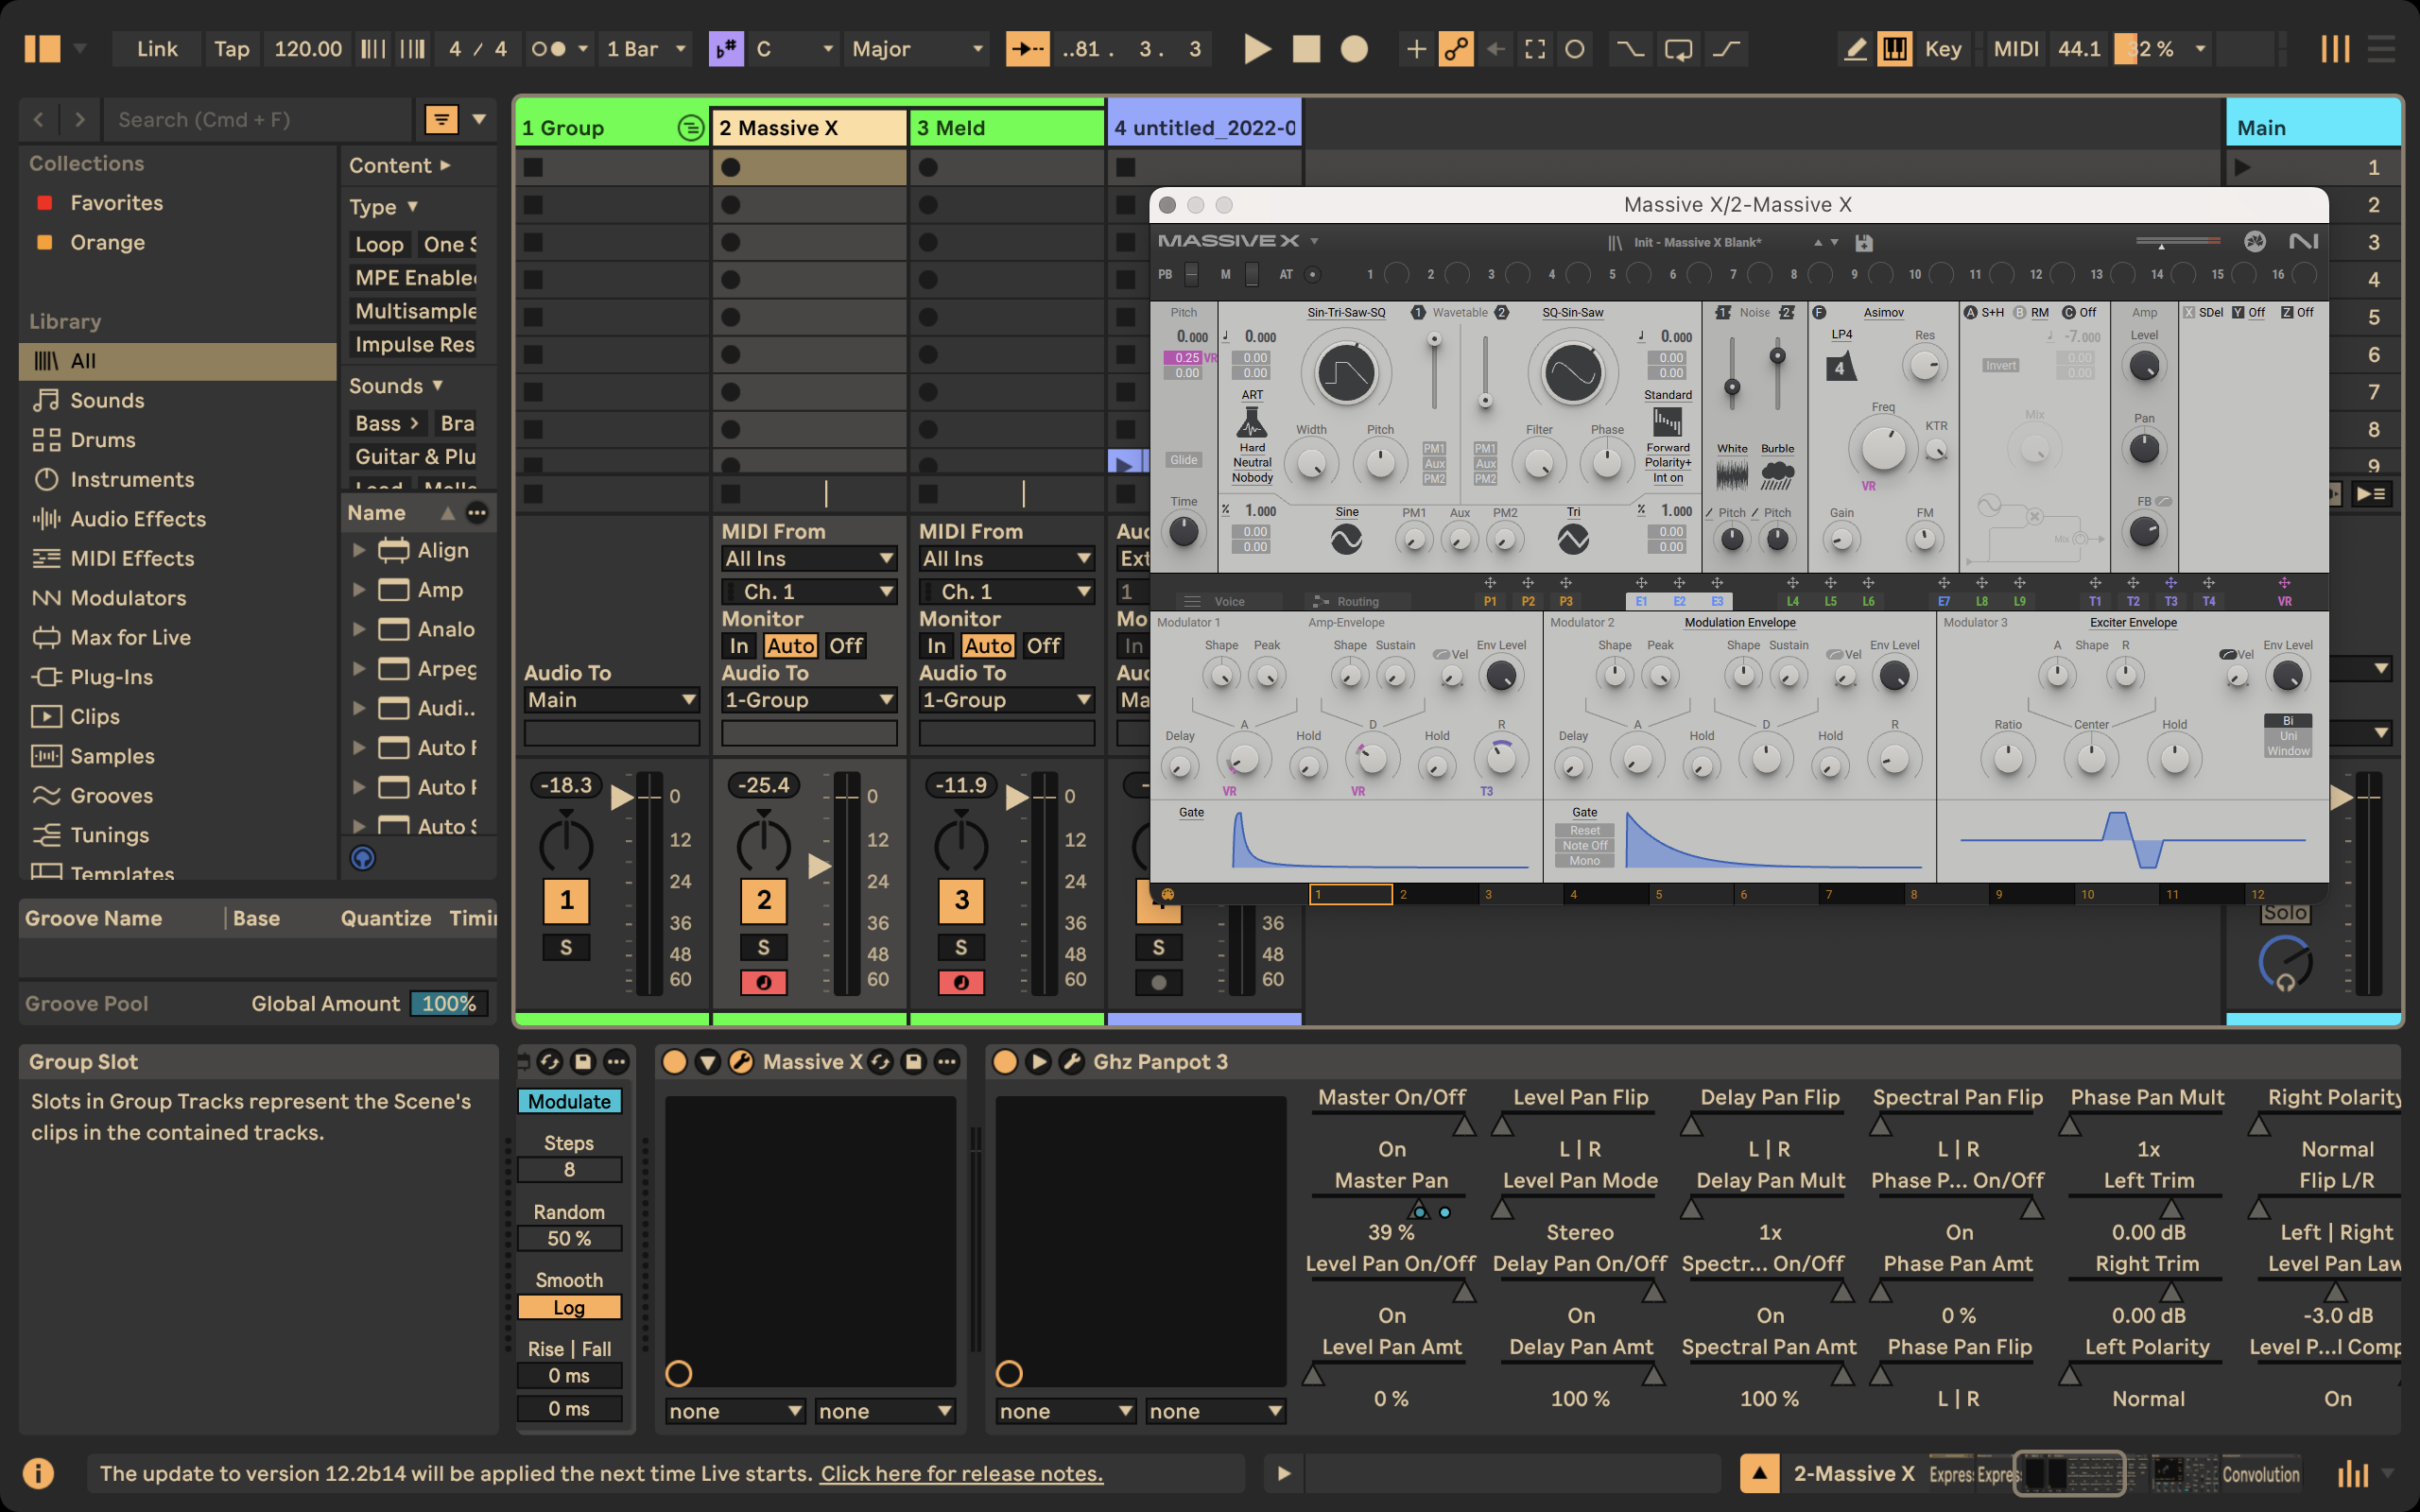
\includegraphics[width=11.3cm]{images/live-midi-particles.png}}
    \end{figure}
    The sound design of each ``cosmic ray'' sought to mirror cosmic particles' real-life nature as described in section~\ref{sec:intro}; thus, each generated blip of sound corresponding to an \textsc{led} activation was comprised of two sonic parts:
    \begin{enumerate}
        \item   a transient, relatively intense, percussive burst of filtered white noise (representing a high-energy progenitor particle impacting the atmosphere), followed by
        \item   a diffuse background tail: a harmonic thrum, naturally swelling and lulling in intensity based on the density of subsequent pulses (representing the diffusion of the progenitors' energy throughout the atmosphere).
    \end{enumerate}
    
    One further aspect of development was the inclusion of refractive materials to catch and re-direct light inside the volume of the box (which otherwise felt somewhat empty). We opted for very cheap and accessible materials such as clear plastic plates to mock up what a more refined centerpiece sculpture might look like in the future (\cref{fig:scattering}).

    \begin{figure}[h]
        \floatbox[{\capbeside\thisfloatsetup{capbesideposition={right,center},capbesidewidth=3.5cm}}]{figure}[\FBwidth]
        {\caption{Example configuration with a central refractive sculpture.}\label{fig:scattering}}
        {\includegraphics[width=\linewidth]{images/scattering.png}}
    \end{figure}

    \begin{figure}[h]
        \floatbox[{\capbeside\thisfloatsetup{capbesideposition={right,center},capbesidewidth=3.5cm}}]{figure}[\FBwidth]
        {\caption{Final corner connector design. Cubical, rather than flat.}\label{fig:corner}}
        {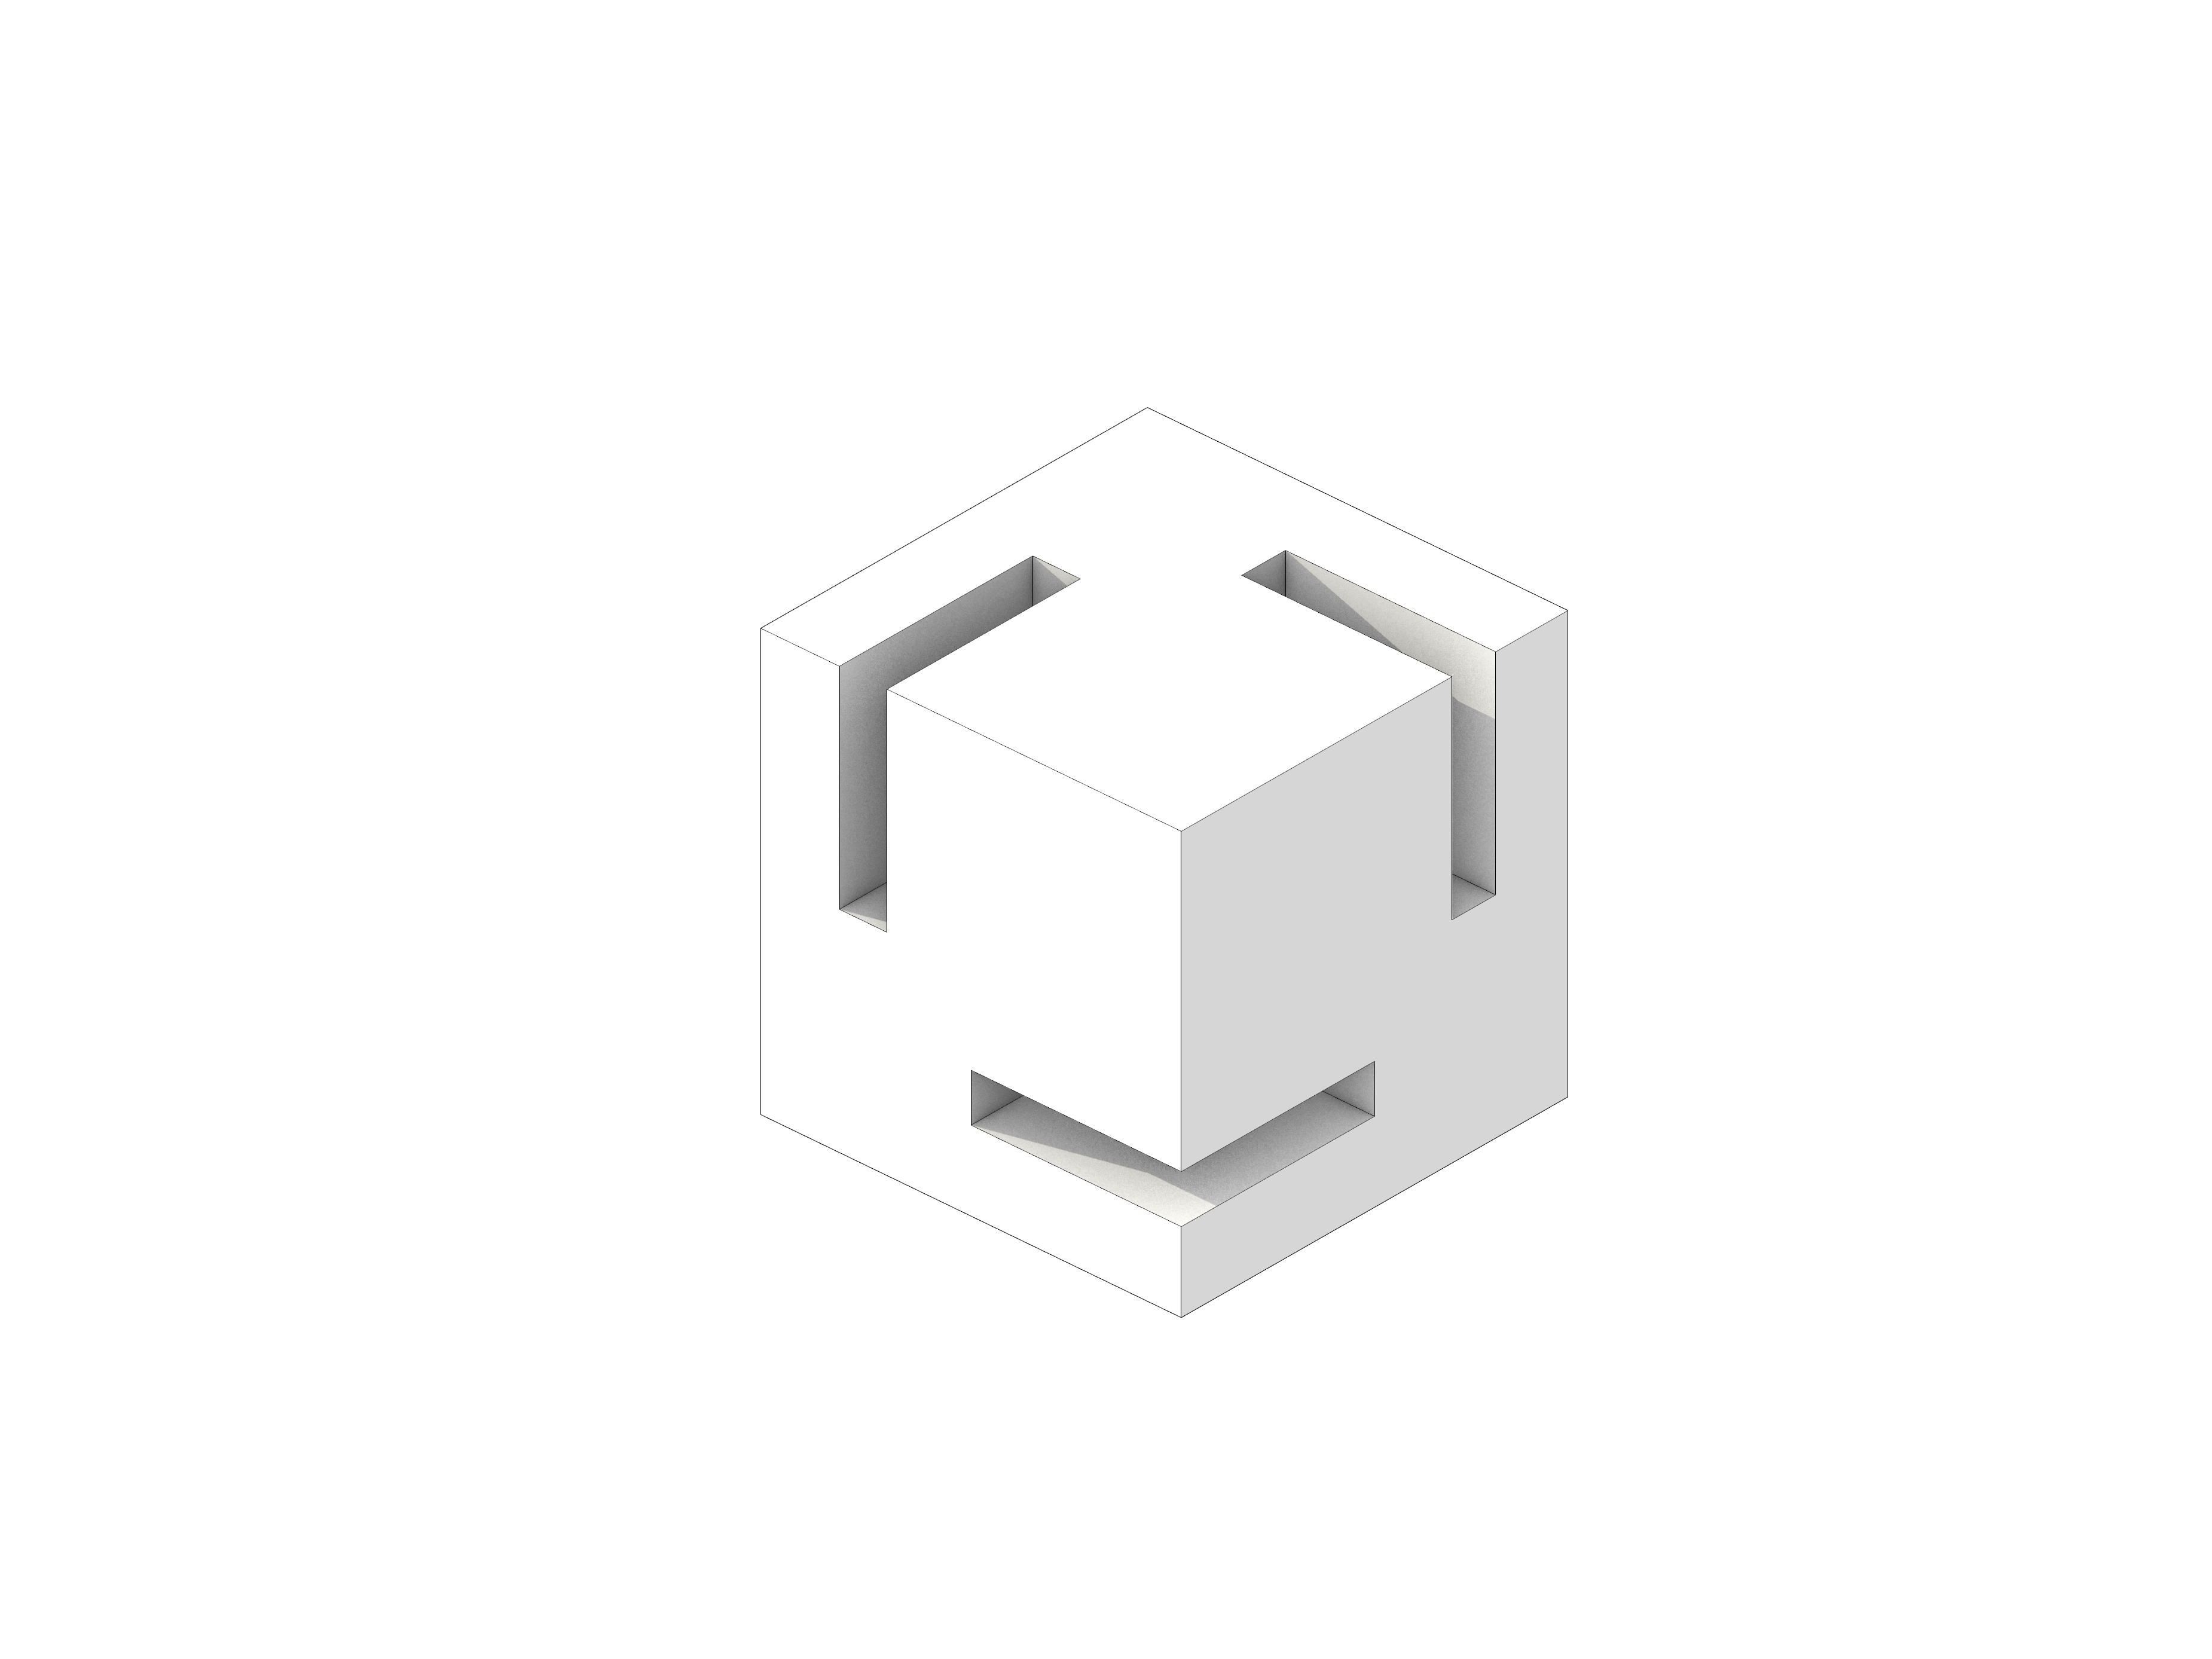
\includegraphics[width=\linewidth]{images/corner.png}}
    \end{figure}

    
    \begin{figure}[h]
        \floatbox[{\capbeside\thisfloatsetup{capbesideposition={right,center},capbesidewidth=3.5cm}}]{figure}[\FBwidth]
        {\caption{Initial mockup. Planned use of a projector would allow for diverse visual effects.}\label{fig:mockup}}
        {\includegraphics[width=8cm]{images/Mock up 1.pdf}}
    \end{figure}
    \begin{figure}[h]
        \floatbox[{\capbeside\thisfloatsetup{capbesideposition={right,center},capbesidewidth=3.5cm}}]{figure}[\FBwidth]
        {\caption{Second generation of corner connectors (exlpoded view) These connectors added a slight gap between panes to allow more light to enter.}\label{fig:exploded}}
        {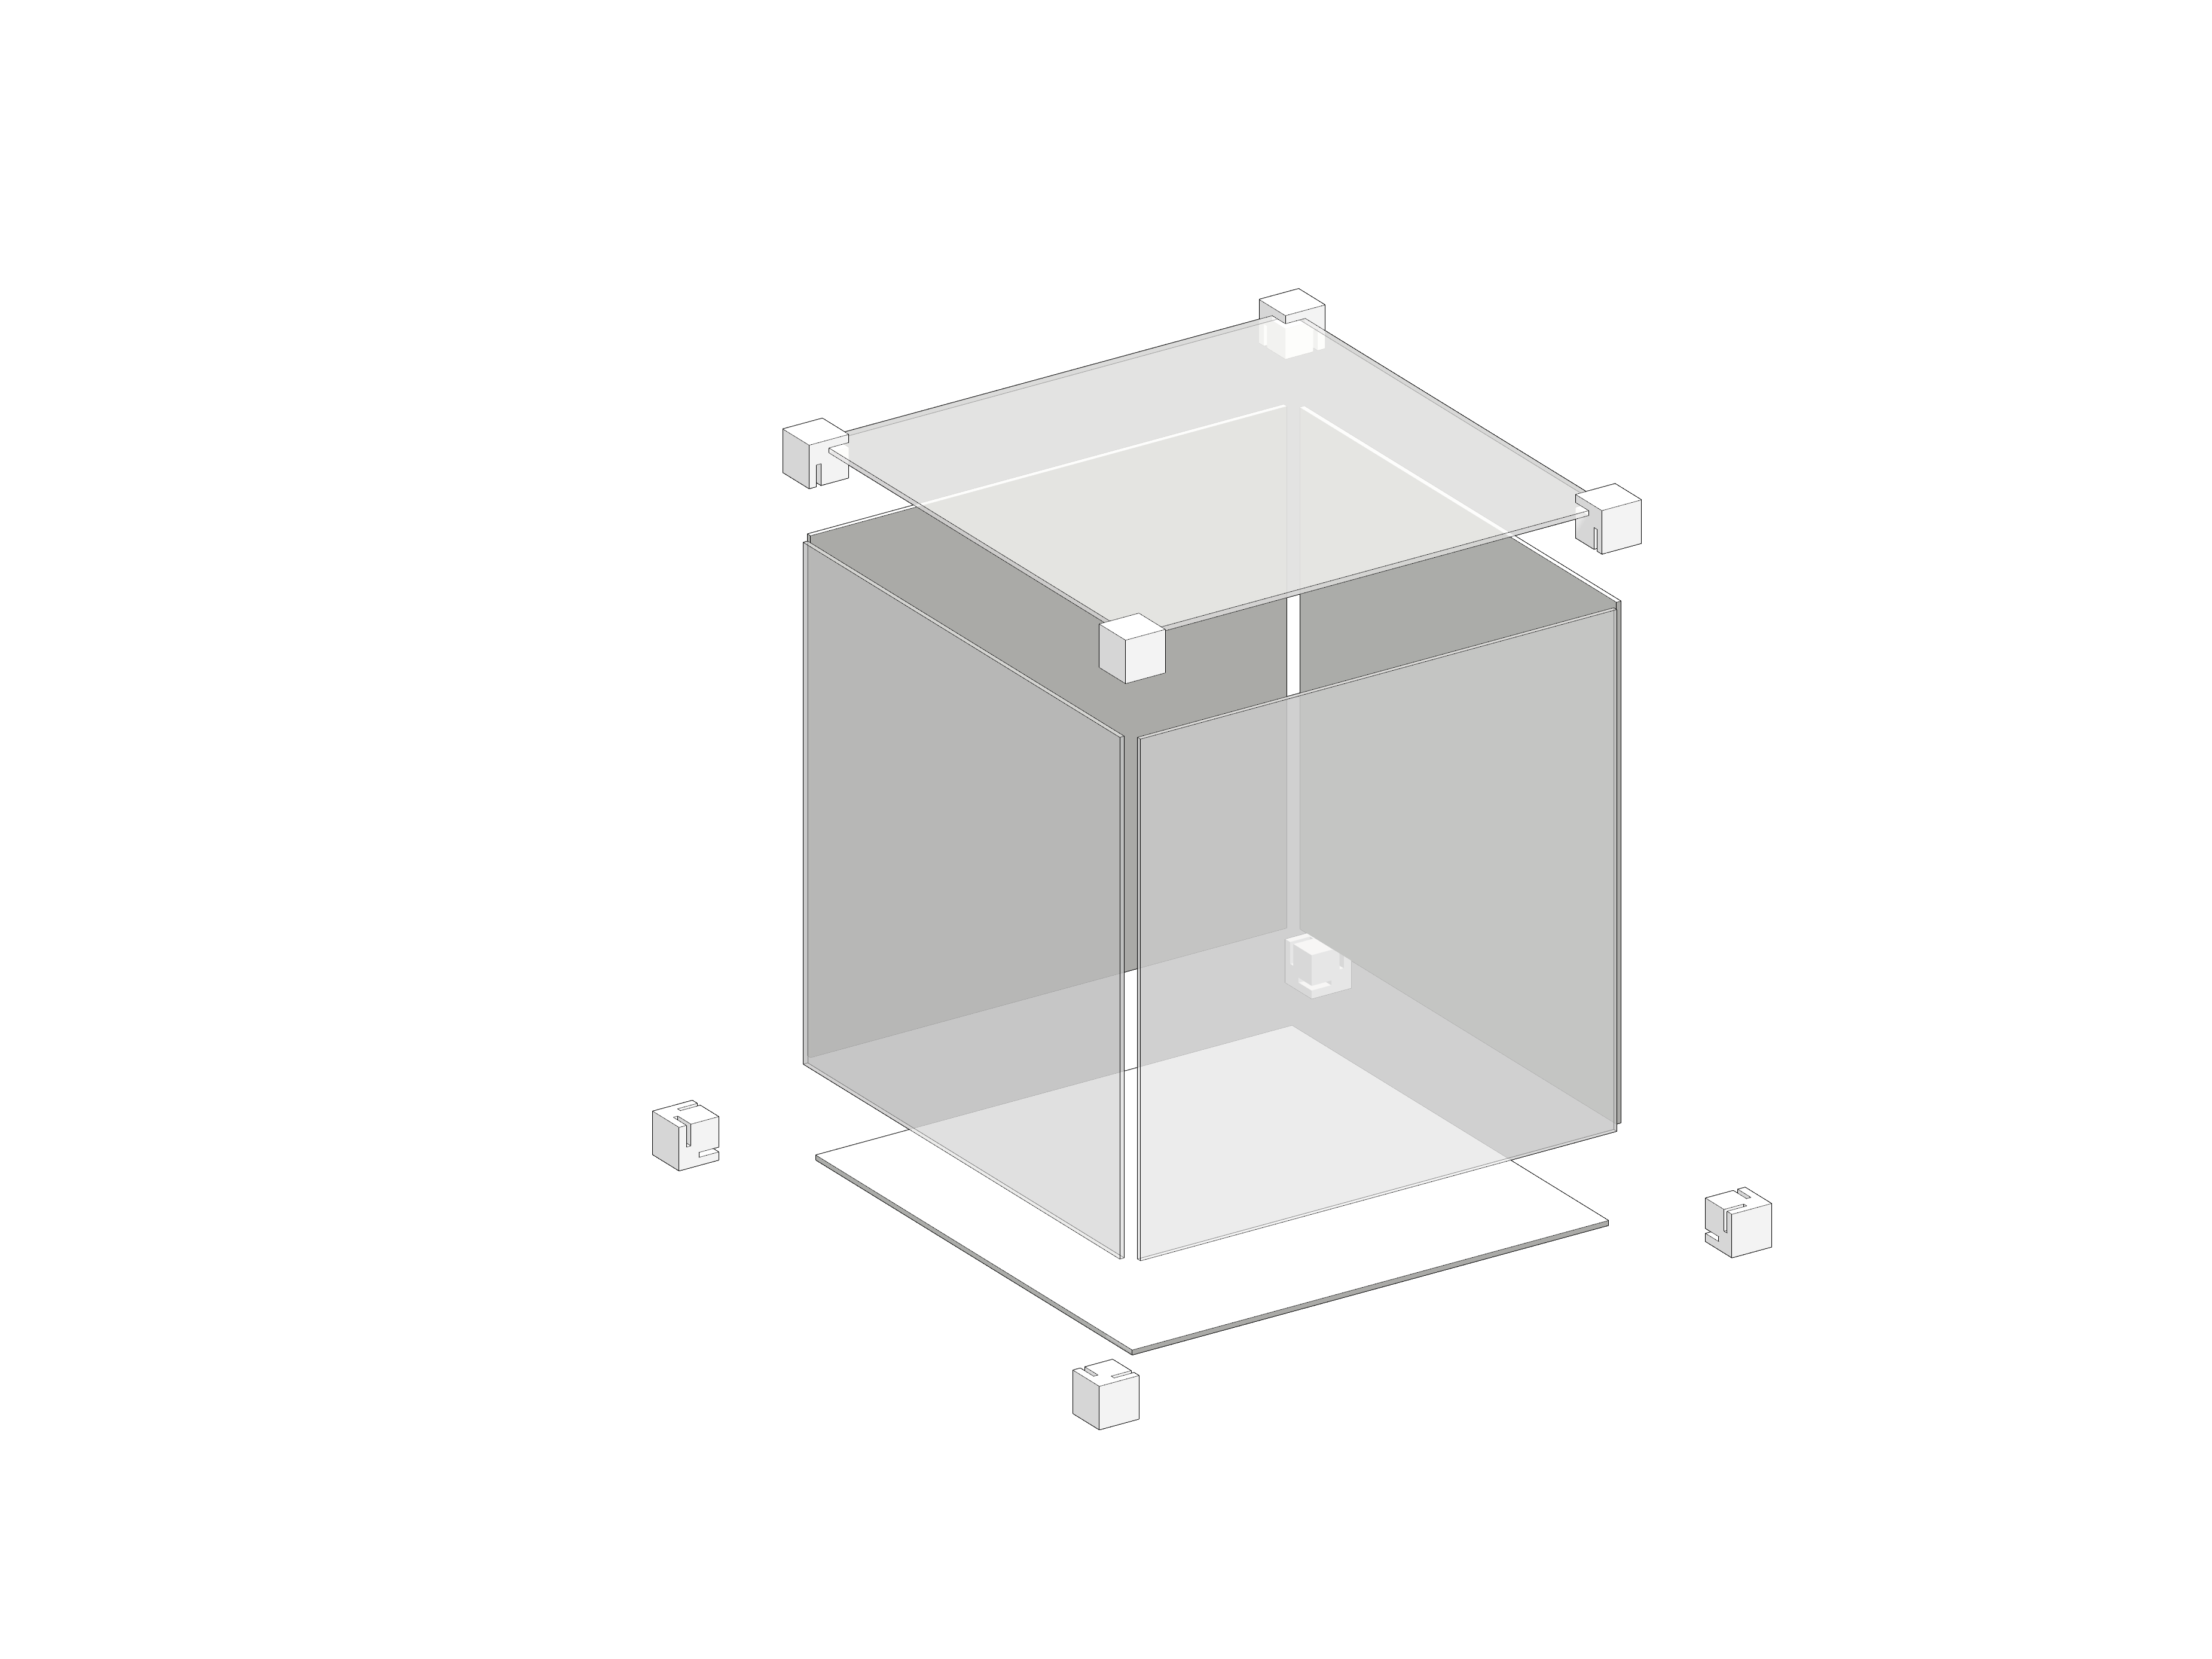
\includegraphics[width=8cm]{images/exploded.png}}
    \end{figure}

    The final prototype was a cubic-foot box consisting of eight corner joints connecting six single-square-foot plexiglass panels (three opaque and three permeable mirrors), a central refractive sculpture, an Arduino–\textsc{led} circuit for light and \textsc{midi} generation, and a computer and headphones for audio synthesis and playback.
    

    
    \pagebreak
    \section{Evaluation \textsc{\&} reception}

    \subsection{Essential successes (roses)}

    We were proud to have created a well-received design, despite
    room for improvement. Visiting judges at review days were generally impressed with the immersive aspects of the experience, citing the audio and general framing of the box prototype as pleasant and well-executed. At \textsc{eur}ē\textsc{ca}, we were awarded second place in the interior architecture and design division for our project and presentation, and the judges seemed very pleasantly surprised.

    A lesson from this: setting viewers' expectations very low at the outset (see the limp towel unceremoniously draped over our box in \cref{fig:eureca}) can lead to subversive and unexpected delight when the immersion of the experience begins. The audio allowed for this extra level of immersion—it was one of the most beneficial aspects of our design; hearing should be treated with care in future iterations, as it adds to the accessibility and immersion of the experience.
    \begin{figure}[h]
        \floatbox[{\capbeside\thisfloatsetup{capbesideposition={right,bottom},capbesidewidth=3.5cm}}]{figure}[\FBwidth]
        {\caption{\textsc{eur}ē\textsc{ca} group photo with our project. \textit{Left to right:} Jaedyn, Eliza, Micah, Hunter.}\label{fig:eureca}}
        {\rotatebox[origin=c]{-90}{\includegraphics[width=13.03cm, rotate=90deg]{images/eureca.jpeg}}}
    \end{figure}

    Further, the successful implementation of modular 3d-printed connectors was a great success. At first, we were having issues with stability, but we learned that using ``glue dots'' added the exact right amount of stability to hold everything together.
    
    \subsection{Future opportunities (buds)}
    Before selecting our final design's lighting schema, we entertained several alternatives. One idea we found particularly interesting was the prospect of using blackbody lighting, such as from incandescent filaments, in place of our addressable \textsc{led}s. This kind of lighting more closely approximates ``natural'' blackbody radiation (such as from the sun). The use of incandescent filaments in future iterations could add depth and warmth to future designs, although could pose a greater challenge to the construction process. 

    Additionally, the user interaction from our ``particle density'' knob can be counted as a success, although the tactile experience should be given more attention if used in the future. The limp and unsatisfying breadboard potentiometer did the job valiantly, but it was not the nicest to interface with.
    
    Further, the inclusion of a refractive central sculpture was well-received by many viewers and reviewers, but could be an area of focus for improvement in terms of material quality and positioning within the box.
    
    One other opportunity for innovation and expansion on this concept is the \textit{direct} inclusion of cosmic phenomena in the design, whether it be through cosmic triggers or some other means. The closer future iterations can get to visualizing or experientializing the \textit{real thing}, directly, the better. Arguably, the most awe-inspiring experience one can have with cosmic rays is \textit{directly} seeing evidence of them; if this aspect can be somehow emphasized in future iterations of the project, successes of this iteration could be strongly amplified.
    

    \subsection{Challenges (thorns)}

    This being a prototype, material quality and selection was not deeply considered. Experimenting with more materials (beyond the realm of plastics) could add a great degree of polish to this concept. Precisely machined metallic connectors and a greater attention to lighting selection are among the many potential improvements to the material and aesthetic quality of our design.
    
    Additionally, one of the greatest challenges to our success was finding a direct way to connect our exploration with the real-world phenomenon of cosmic radiation. Loose symbolic representations of cosmic phenomena, along with the \textit{ability} (which was never manifested) to connect a cosmic trigger to the setup were sufficient qualities for this iteration, but future projects should lend this matter very close attention.
    
    
    \pagebreak
    \section{Next steps}

    \textsc{we believe} that a focus on material quality and design simplicity with sound choices and aesthetic execution will allow for the cosmic phenomena to be the focal point of the design. Attention to expanding multisensory experience of cosmic rays should be prioritized. We envision our concept expanded to a room scale, with lighting events triggered by cosmic ray detection in \textit{real time}, further grounding the concept in actual events from space.

    \begin{figure}[h]
        \floatbox[{\capbeside\thisfloatsetup{capbesideposition={right,center},capbesidewidth=3.5cm}}]{figure}[\FBwidth]
        {\caption{Vision of a future exhibit. Fully mirrored rooms allow designers to play with expansive artificial spaces to represent the pervasiveness and vastness of cosmic phenomena.}\label{fig:scattering}}
        {\includegraphics[width=11.5cm]{images/CosmicRaysRendering.pdf}}
    \end{figure}
    
\clearpage
\AddToShipoutPictureBG*{%
  \put(220,-620){\scalebox{-1}[1]{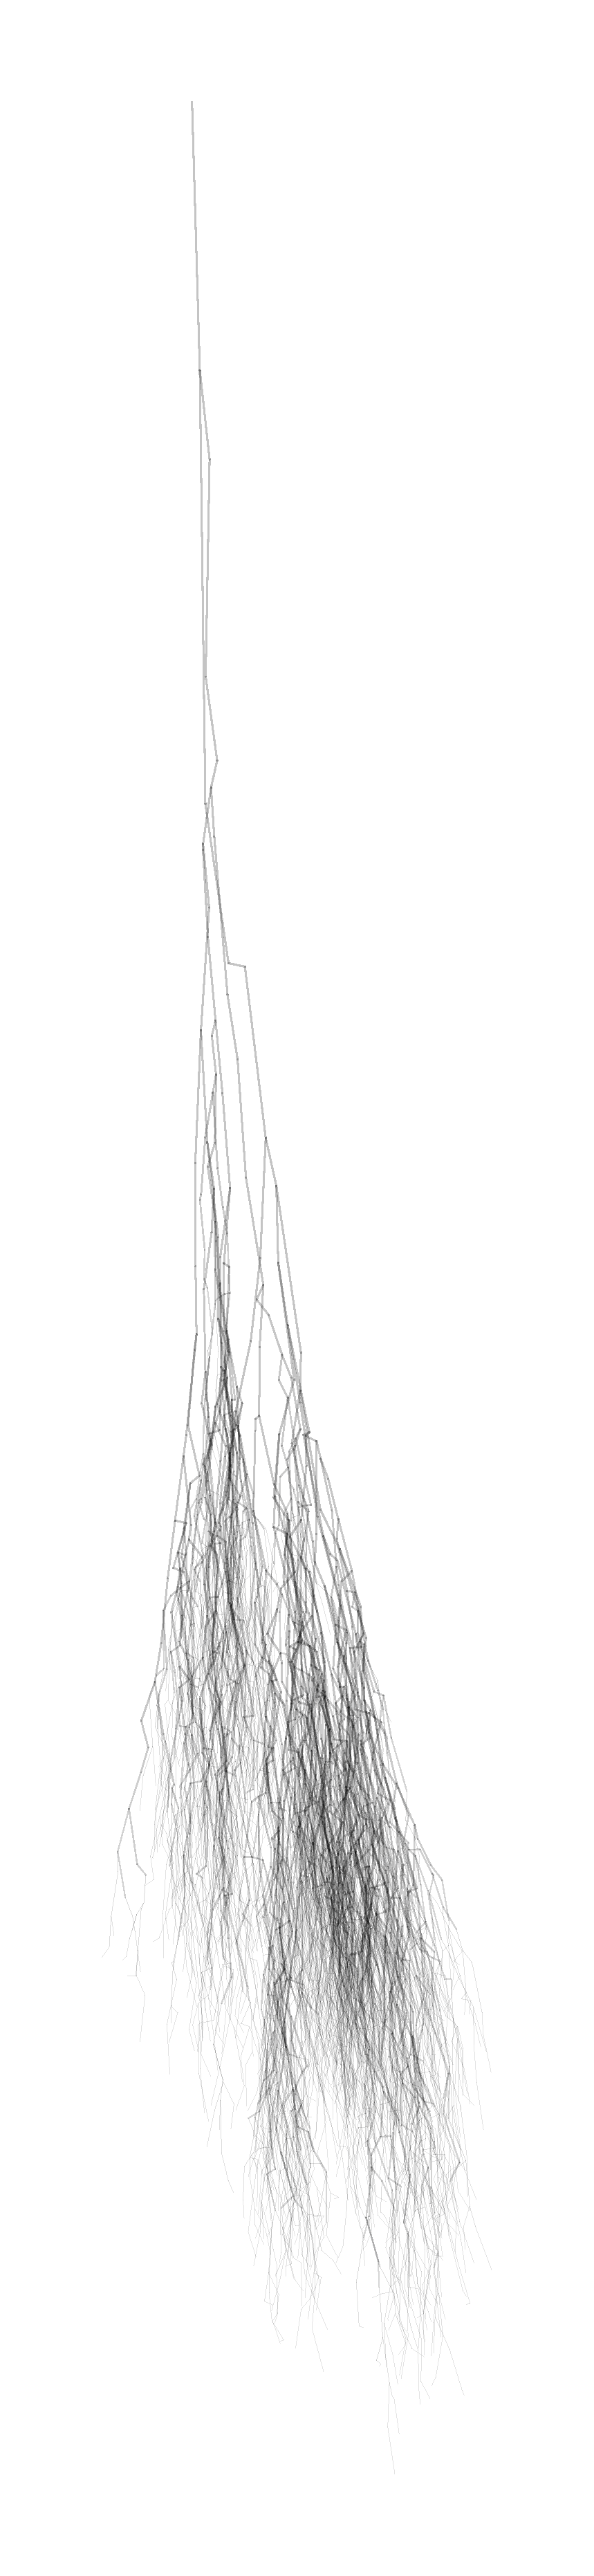
\includegraphics[height=250em]{images/shower.pdf}}}%
}
\thispagestyle{empty}
\printbibliography
\clearpage
\AddToShipoutPictureBG*{}  % Clear background for next pages

\end{document}
